\section{Input Analysis}

In this section we analyze the data that has been collected. One data set contains arrival times of vehicles from the last month. An other file has numbers of the amount of fuel a was needed by a vehicle. 

\subsection{Arrival Times}

We have a raw data set containing arrival times of vehicles at the station over a course of 30 days. 
A histogram of the number of arrivals over time is shown in Figure \ref{fig:histogram-arrivals}. 
Fitting analysis has shown that a Beta distribution is the best fit for this data, a summary of the Fit all functionality of Arena Input Analyzer is shown in Table \ref{tab:fitallarrivals}. Fitting a single distribution might not be very useful though. We can see that the busiest periods are around 7 AM and 6 PM. So it would be more interesting to fit distributions around these times. 

\begin{figure}[h]
	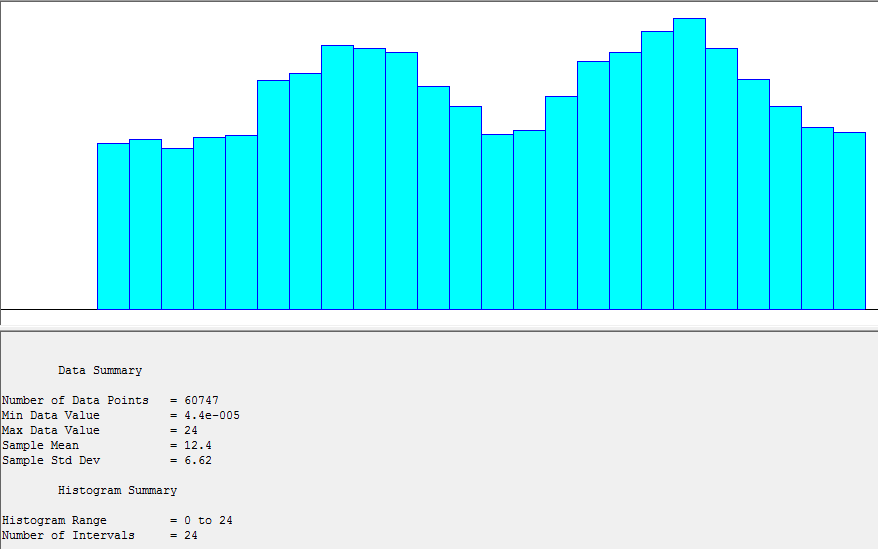
\includegraphics[width=\textwidth]{images/histogram-arrivals.PNG}
	\caption{Histogram of arrival times, each of the 24 intervals represents one hour.}
	\label{fig:histogram-arrivals}
\end{figure}

\begin{table}[h]
	\centering
	\begin{tabular}{r | l}
		Function  &     Sq Error\\
		\hline
		Beta       &  0.000889\\
		Uniform     & 0.00141\\
		Normal       &0.00507\\
		Gamma        &0.00703\\
		Erlang       &0.00712\\
		Triangular   &0.00915\\
		Lognormal    &0.0122\\
		Exponential  &0.0143\\
		Weibull      &0.107	
	\end{tabular}
	\caption{Fit all summary of Arena Input Analyzer on Arrivals\_(13).dst}
	\label{tab:fitallarrivals}
\end{table}

Figure \ref{fig:histogram-inter-arrivals} shows a histogram of the time difference between successive arrivals. This data fits a poisson distribution with mean .. 

\begin{figure}[h]
	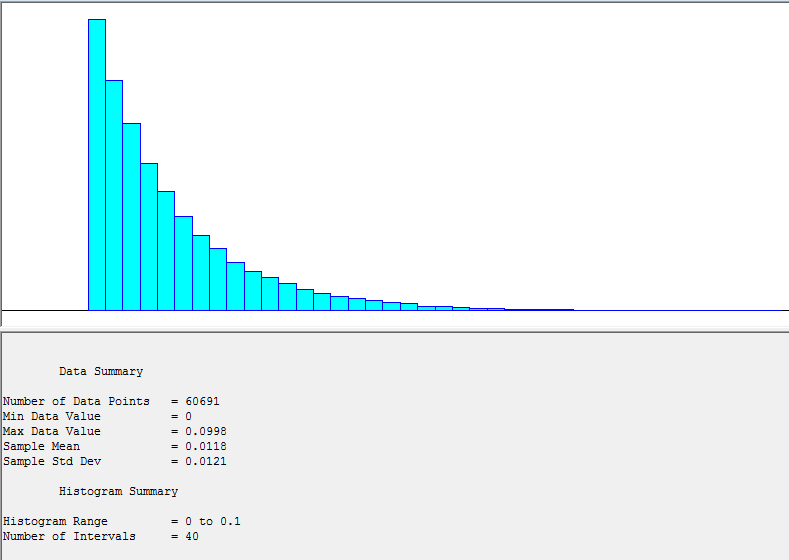
\includegraphics[width=\textwidth]{images/histogram-interarrivaltimes.PNG}
	\caption{Histogram of inter arrival times, 40 intervals over the range 0 - 0.1 hours.}
	\label{fig:histogram-inter-arrivals}
\end{figure}

\subsection{Fuel Amounts}

In the fuel amounts dataset, we see a clear difference between cars and trucks.
A histogram of the fuel amounts is shown in Figure \ref{fig:histogram-amounts-unfiltered}, here the high peak corresponds to fuel needed by cars, the lower bars correspond to fuel needed by trucks.
In Figure \ref{fig:histogram-amounts-filtered}, a histogram is shown of only the car data, here the maximum data value has been set to 100.
In Table \ref{tab:fitallamounts} summaries of \textit{Fit all} of the Arena Input Analyzer are shown.
The car data in itself is best described by a normal distribution, all data is best described by a Lognormal distribution, where all car data is compressed into one bar of the histogram.

\begin{figure}[h]
	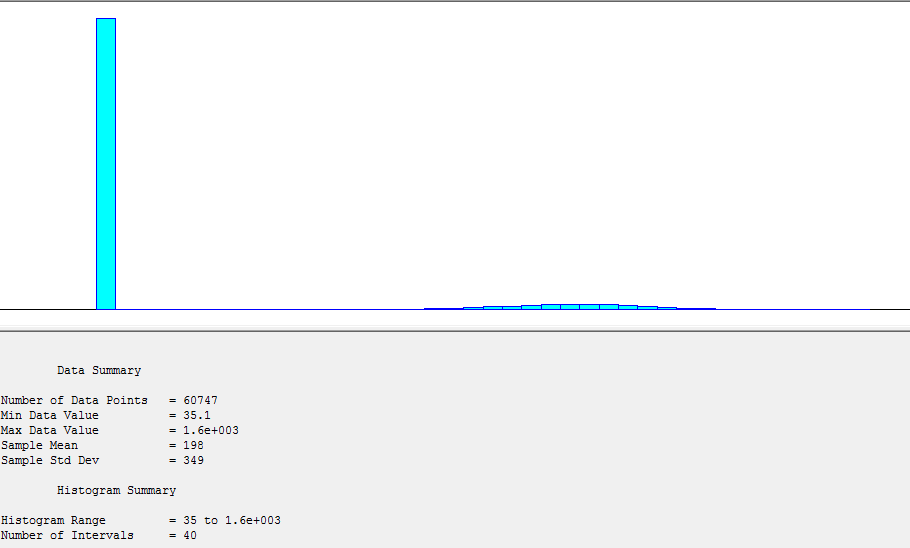
\includegraphics[width=\textwidth]{images/histogram-amounts-unfiltered.PNG}
	\caption{Histogram of used fuel amounts, 40 intervals, on the raw data}
	\label{fig:histogram-amounts-unfiltered}
\end{figure}

\begin{figure}[h]
	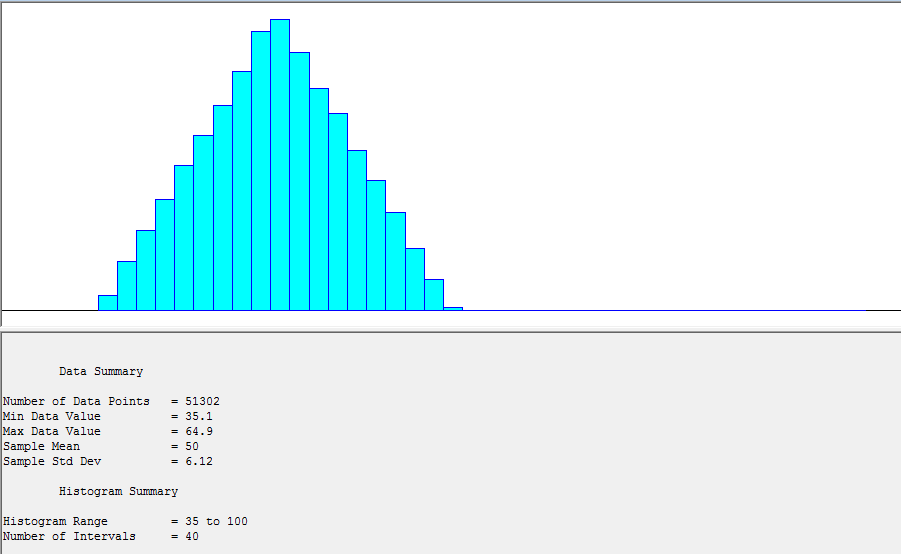
\includegraphics[width=\textwidth]{images/histogram-amounts-filtered.PNG}
	\caption{Histogram of used fuel amounts, 40 intervals, when maximum data value was set to 100 litres.}
	\label{fig:histogram-amounts-filtered}
\end{figure}

\begin{table}[h]
	\parbox{.3\linewidth}{
		\centering
		\begin{tabular}{r | l}
			Function  &     Sq Error\\
			\hline
			Lognormal    &0.0976\\
			Weibull      &0.118\\
			Beta         &0.226\\
			Gamma        &0.285\\
			Exponential  &0.473\\
			Erlang       &0.473\\
			Normal       &0.668\\
			Triangular   &0.679\\
			Uniform      &0.69\\
		\end{tabular}
		\caption{Fit all summary of Arena Input Analyzer on Amounts\_(13).dst}
		\label{fitallamountsunfiltered}
	}
	\parbox{.05\linewidth}{\ }
	\parbox{.3\linewidth}{
		\centering
		\begin{tabular}{r | l}
			Function  &     Sq Error\\
			\hline
			Normal       &0.000575\\
			Weibull      &0.000587\\
			Beta         &0.00239\\
			Erlang       &0.00387\\
			Gamma        &0.00411\\
			Lognormal    &0.00888\\
			Triangular   &0.0277\\
			Exponential  &0.0397\\
			Uniform      &0.0471\\
			
		\end{tabular}
		\caption{Fit all summary of Arena Input Analyzer on Amounts\_(13).dst with maximum amount set to 100}
				\label{fitallamountsfilteredcars}
	}
	\parbox{.05\linewidth}{\ }
	\parbox{.3\linewidth}{
		\centering
		\begin{tabular}{r | l}
			Function  &     Sq Error\\
			\hline
			Normal       &4.18e-005\\
			Weibull      &0.00062\\
			Lognormal    &0.00123\\
			Erlang       &0.00215\\
			Gamma        &0.00219\\
			Beta         &0.00276\\
			Triangular   &0.0201\\
			Uniform      &0.0454\\
			Exponential  &0.0594
			
		\end{tabular}
		\caption{Fit all summary of Arena Input Analyzer on Amounts\_(13).dst with minimum amount set to 100}
		\label{fitallamountsfilteredtrucks}
	}
	\caption{Summaries of \textit{Fit all} of Arena Input Analyzer, all with 40 intervals}
	\label{tab:fitallamounts}
\end{table}



